\documentclass{article}
\usepackage[utf8]{inputenc}

\usepackage[margin=1in]{geometry}
\usepackage{hyperref}
\usepackage{graphicx}
\usepackage{ulem}

\usepackage{titlesec}

\usepackage{float}
\usepackage{caption}
\usepackage{subcaption}


\setcounter{secnumdepth}{4}
\setcounter{tocdepth}{4}
\titleformat{\paragraph}
{\normalfont\normalsize\bfseries}{\theparagraph}{1em}{}
\titlespacing*{\paragraph}
%{0pt}{3.25ex plus 1ex minus .2ex}{1.5ex plus .2ex}
{0pt}{1.0ex plus 1ex minus .2ex}{0.1ex plus .2ex}

\newcommand{\name}{ECW\ }
\newcommand{\nameNospace}{ECW}
\newcommand{\namep}{ECW.}

\renewcommand{\labelenumii}{\theenumii}
\renewcommand{\theenumii}{\theenumi.\arabic{enumii}}
\renewcommand{\theenumiii}{\theenumii.\arabic{enumiii}}

\usepackage{fancyhdr}
\pagestyle{fancy}

\lhead{ Responsible: Alexander Ekman, Linnea Johnsson, and David Ravanelli \\ Date: \today}  \rhead{Document number: PUSS21419 \\ Version: 1.5}
\renewcommand{\headrulewidth}{0.5pt} 


\title{PFR - Project Final Report}
\author{Team 1}

\begin{document}

\date{}
\maketitle
\thispagestyle{fancy}
\newpage

\section*{Revision History}
\begin{table}[h]
    \centering
    \begin{tabular}{|l|l|p{55mm}|p{35mm}|}
    \hline
    Date & Version & Description & Author \\ 
    \hline\hline 
    2021-10-13 & 1.0 & Section headings and structure & David Ravanelli, Linnea Johnsson, Alexander Ekman  \\
    \hline
    2021-10-13 & 1.1 & First draft and outlines of all sections & David Ravanelli  \\
    \hline
     2021-10-14 & 1.2 & Rough version of all the sections & David Ravanelli \\
    \hline
     2021-10-16 & 1.3 & Completed Phase 1 and 2 sections & David Ravanelli \\
    \hline
      2021-10-18 & 1.4 & Completed Phase 3 section & David Ravanelli \\
    \hline
    2021-10-18 & 1.5 & Draft Section of the Forgotten Issues & Alexander Ekman \\
    \hline
    \end{tabular}
    \label{tab:history}
\end{table}
\newpage

\begin{thebibliography}{widest entry}

    \bibitem{PH} "Programvaruutveckling för Stora System Projekthandledning 2021", Chapter 9, Institutionen för Datavetenskap Lunds Tekniska Högskola, Lunds Universitet, 26 August 2021
    
    \bibitem{SDP} "SDP - Software Development Plan, Team 1 - ETSN05", Alexander Ekman and Linnea Johnsson, version 1.3
    
    \bibitem{PRD} "PRD - Product Requirements Document, Team 1 - ETSN05", Alexander Ekman and Linnea Johnsson, version 1.21
    
    \bibitem{SPF1} "SPF1 - Software Product Features 1, Team 1 - ETSN05"
    
    \bibitem{SP1} "SP1 - Sprint Planning 1, Team 1 - ETSN05"
    
\end{thebibliography}
\newpage

\tableofcontents
\newpage

%information från PH: I samband med projektet ska data samlas in för att bl.a. följa upp nedlagd tid och antal fel. Denna information är en bra grund att ha då man ska starta ett nytt projekt, och dokumenteras därför i en slutrapport. Genom att analysera denna rapport kan man då göra en bra planering både med avseende på tid i allmänhet och resurser som behövs för att rätta de fel som man trots allt gör. I slutrapporten är det således viktigt att man sammanställer insamlad data på ett lämpligt sätt samt att man drar slutsatser utifrån dessa. 
%För alla data som skattades i tidplanen(I SDP!) ska verkligt utfall redovisas. Om tidplanen uppdaterats under projektets gång så ska jämförelse ske med de ursprungliga värdena(Det fick vi ej göra). Eftersom dokumentet skrivs innan sista veckan är färdig så finns inte metricsdata tillgänglig för sista veckan i projektet. Detta kan lösas antingen genom att inte ta med sista veckan i analysen, eller genom att använda skattade värden för sista veckan. 
%Slutrapporten ska omfatta max 20 sidor (exklusive försättsblad, innehålls- förteckning, etc.). Målgruppen för en slutrapport har ofta ont om tid, samtidigt som det är viktigt att rapporten blir läst. Alltså ska omfånget vara begränsat och gäller att välja vad man presenterar och sättet man gör det på.

\section{Introduction}
%what will this report go through?
This report will present an evaluation and overview of the project, its methodology, and its deliverables. The purpose of this is to provide useful information on how what went well/bad, why, and how to promote/avoid these in future projects. Lastly, the conclusion of this evaluation will be summarized for easy use in future projects.

\section{Phase 1}
\subsection{Historical overview}
%Vad är det som har hänt? Siffror, tabeller och diagram. Jämförelser och uppvisande av data.

Phase 1 was the specification phase where the product requirements, specifications, and project planning was determined and documented in the Product Requirement Document (PRD)\cite{PRD}, and the Software Development Plan (SDP)\cite{SDP}. In this phase the product backlog (SPF1)\cite{SPF1} and the first Sprint Planning (SP1)\cite{SP1} were also produced. 

At the start of the phase, the whole development team met and discussed possible epics, user stories, and issues for the project. This discussion took of from drafts of the PRD \cite{PRD}. This discussion lead to a list of issues that was prioritized and added to the SPF1 \cite{SPF1}. During the same meeting the team also decided on which items to bring from the SPF1 into the first sprint, this is documented in the SP1\cite{SP1}. 

The project team was then split into three different internal teams: back end, front end and algorithm. Sprint 1 had not started yet, but the teams were encourage to met up and get to know each other. The main purpose for these first internal team meetings was to plan ahead for the upcoming sprint. In the meantime the project owners planned the structures of the mentioned documents and the scrum master (SM) started to research and collect the necessary metric equipment's. 

The phase ended with a formal review where the team got feedback on the written documents that were produced. Most of the feedback was on document details but also a little bit about the team structure. We had missed to show who will be responsible for meetings, taking notes, creating action points and code reviews.

\subsection{Evaluation \& suggestions of improvements }
%Varför ser det ut som det gör? Analys av de siffror man samlat in. Varför tog det så lång tid i den fasen? Varför blev den modulen så snabbt klar?
%Hur ska man göra för att förbättra de positiva trenderna och få bort de negativa trenderna? Process förbättring mm.

\subsubsection{Data and team structure}
For this phase we didn't have any data to collect since we did not have access to time reporting yet. Furthermore, no code implementation was done on issues since sprint 1 had not started. The only work done, except for common course work, was project documentation. For these deliverables, one can mostly look on the time planned, time spent and the quality of the documents produced. 

Regarding the team structure, feedback showed that the project team appreciated that we split them into sub teams. This made sure that each developer was being utilized where they felt useful and could use their skills to their full extent. Also, this made the developers feel more confident about the upcoming work. 

From the phase 1 review feedback, we improved the missing details in our documents and also clearer outlined the team's structure and responsibilities. The scrum master would be responsible for all the meetings, taking notes and creating action points. This seemed like a good setup since the SM was the most intersected role. The architectures got the responsibility to manage the code reviews, since they had the main responsibility, and overview, of the codes structure and future development plans.

\subsubsection{Phase 1 documentation deadlines in phase 2}

\subsubsection{Project management tools} 
%Förvirringen kring Jira, oneclick, gitlab, epuss osv osv

The project was planned to be managed via Atlassian JIRA, but as the free version only supported 10 developers, our team of 13 had to look for another solution. Multiple other tools were considered, one of them being ClickUp, but since their free version only allowed some objects to be viewed a certain amount of times this tool was also scrapped. A locally managed gitlab server was lastly chosen as both the code repository and the project management tool. This non premium, and locally managed, service was still lacking some features compared to the premium alternatives. We choose E-puss for time reporting. This needed in later phases to be changed to an excel sheet due to a incompatibility between the faculty and E-puss's terms of agreement.

In gitlab's project management tools there were no hierarchical structure for epics, user stories, issues, and sub issues. Instead all entries in the product backlog were added as an issue. Each having a unique ID as X.Y.Z. Where X is the Number of the Epic, Y the number of the user story, and Z the issue number. In this way we were able to organize epics, user stories, and issues in a somewhat hierarchical order. However, since gitlab didn't have the option to sort the list of issues by name, a list in hierarchical order was never available. This version of gitlab also did not provide metrics such as burn down charts, so this had to be produced manually.

In hindsight, we would have opted for prioritizing a project management tool which had more SCRUM functionality. Either by using a paid plan, or setting our group size to 10 in order to use the JIRA software. Though, this would have been against their terms of agreement. Even opting for the official Gitlab instead of a local server could have been beneficial because some functionality such as exporting issue lists and requesting new passwords were not functioning in our version.

Time reporting should have been available from the beginning of the project. This is because the team will then get used to track their time everyday, and increases the chance that they actually keep track of their spent time for the rest of the project. The other argument for having access to time tracking immediately is that it is hard to remember what you did the first weeks, especially since this phase for most students did not include that much project work. Thus, students probably forgot to retrospectively add these time reports. This results in misleading data on how much time the project members has spent on the course, and for the project group (PG) how much time they spent on getting the project started. 

There should also have been a better software available for management tools. For example, in JIRA as discussed earlier, you can automatically assign epics and issues. Now we had to automatically create epics and issues. This wastes a lot of time for the project owner. When the team then adds their own issues there could be a lot of incidents where duplicated issue names are created. This is because it is harder to track the issues manually. Software like JIRA offers automatic tracking of the sprint burndown and velocity chart. Furthermore, the exercises in the course were based on JIRA, meening all project member started the course with learning one tool just to have to switch and learn another, less adequate, tool.

A result of the management tool decision difficulties was that the scrum master had to create a spreadsheet for the upcoming sprint where we could manually track the data. Which once again wastes a lot of time that could be put into helping the team but also made it easier for errors to occur.


\section{Phase 2} %Sprint 1
\subsection{Historical overview}
Phase 2 was the start of Sprint 1. The phase started with a sprint planning meeting on zoom. We estimated that we would be able to finish 91 story points during the sprint, as shown in figure \ref{fig:Burndown1}. The action point from the meeting was that all the sub-teams should meet up and start to plan their given issues. During the phase we had stand up meetings on zoom at the beginning and end of each week. During the days in between we had stand up meetings everyday on slack through text. During a meeting between all the project owners and scrum masters it was decided to use an excel sheet template for time reporting.The second phase ended with a sprint retrospective and also a phase 2 formal review. 

During the sprint retrospective we evaluated the sprint burndown chart as shown in figure \ref{fig:Burndown1}. We recognized that we had underestimated our estimated story points. In the SDP risk analysis section we have outlined what we need to do if we underestimate sprints. With this information we created action points on how to proceed. The amount of issues estimated was wrong but also how many story points that would be completed. We only completed 57 story points. This is a 62.6 percent completion of the originally estimated story points. During the sprint we also added a lot of new issues that we had not accounted for in the original sprint backlog. A total of 119 estimated new story points were added. More than double of our original estimation. This happened very early on and can be seen in the yellow line that spikes up early during the sprint in figure \ref{fig:Burndown1}. During the meeting we also collected data for the team satisfaction as shown in figure \ref{fig:Satisfaction1}. At the phase review we discussed the written documents. From the feedback we were told to adjust some small details.

\begin{figure}[h!]
    \centering
    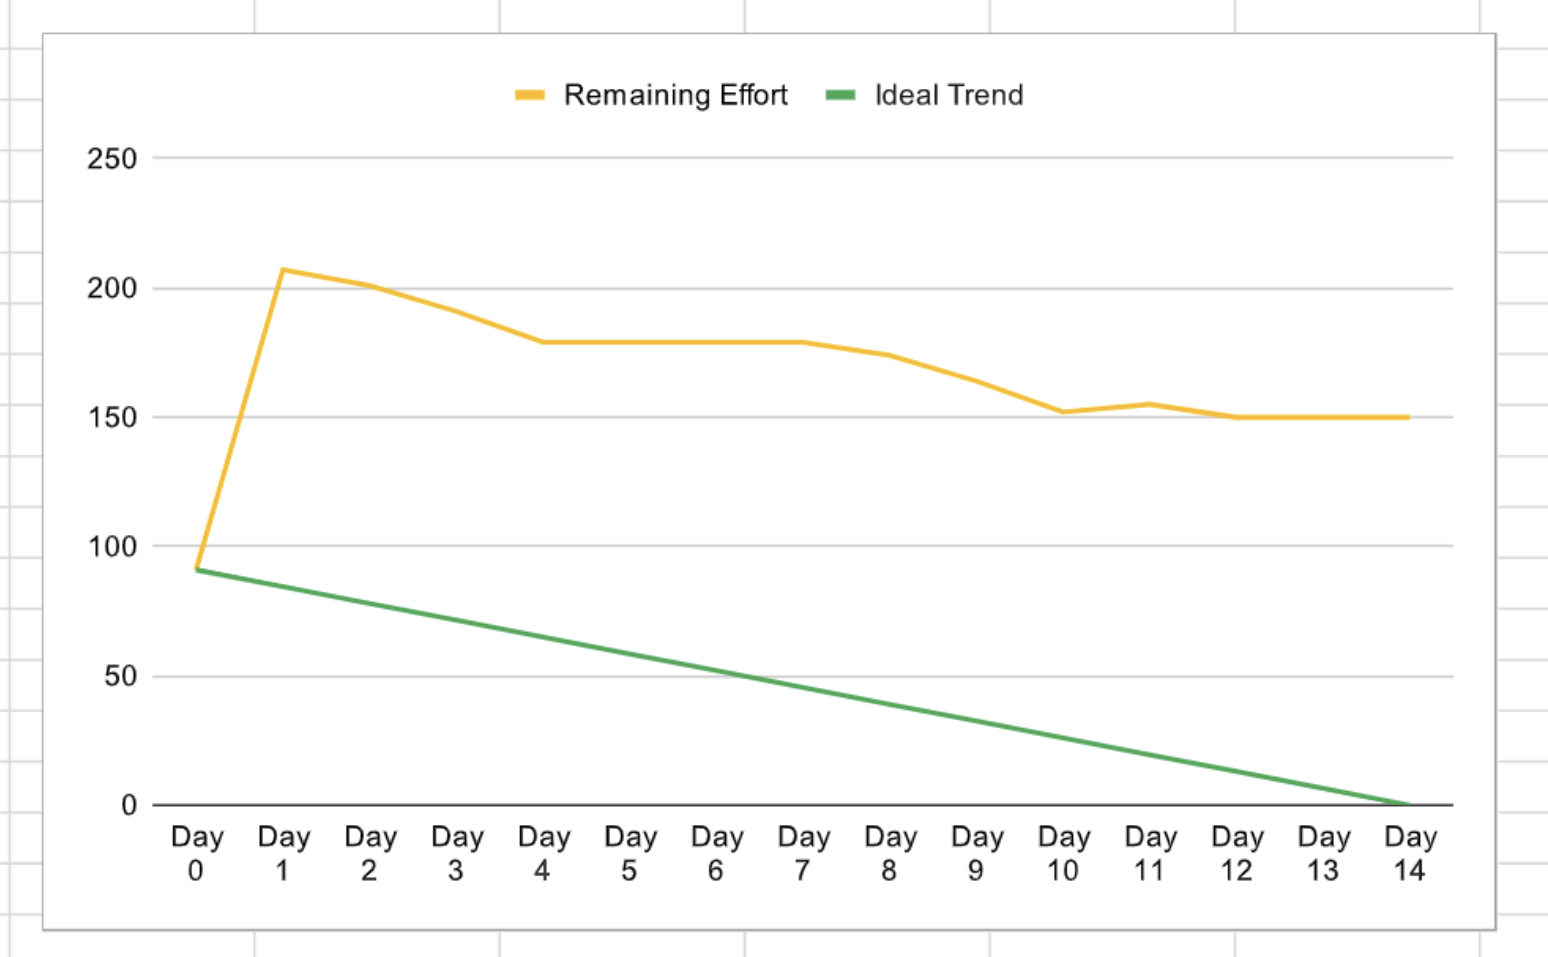
\includegraphics[scale=0.6]{pfrFigures/Sprint1.png}
    \caption{Sprint 1 Burndown chart}
    \label{fig:Burndown1}
\end{figure}

\begin{figure}[h!]
    \centering
    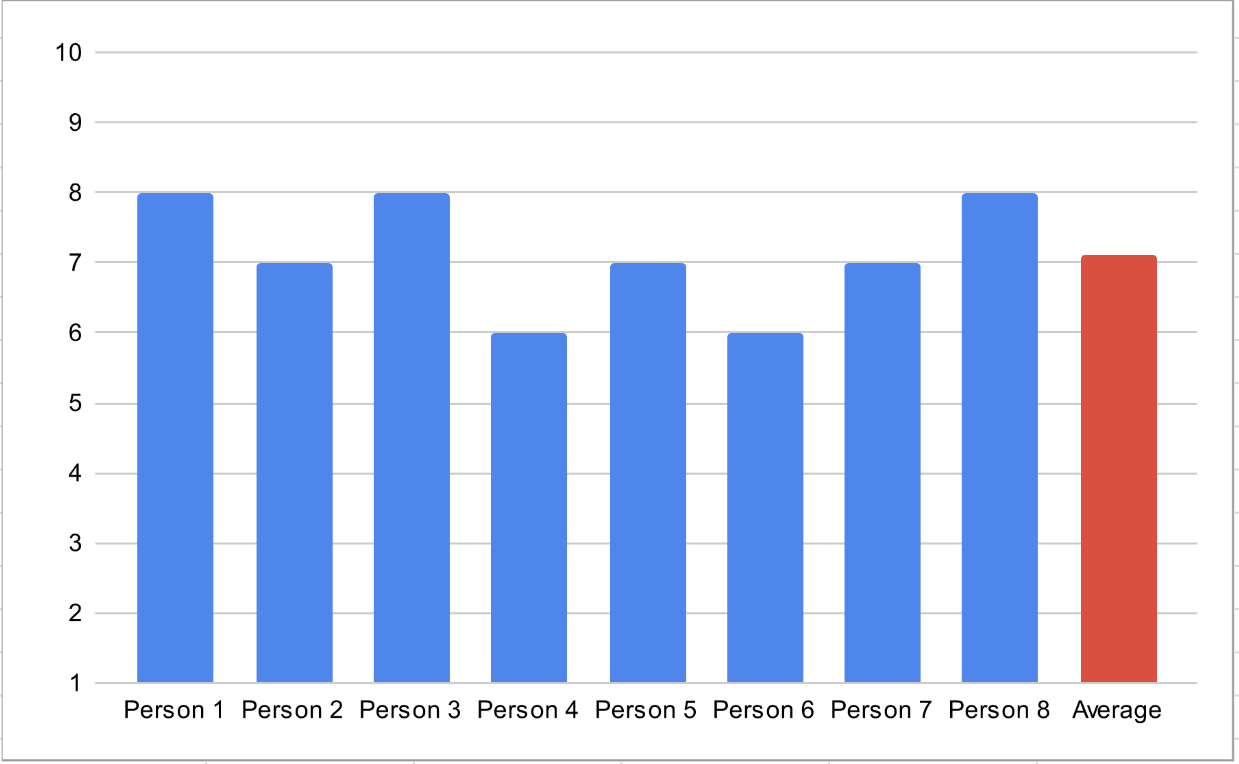
\includegraphics[scale=0.6]{pfrFigures/TeamSatisfaction1.png}
    \caption{Sprint 1 Team Satisfaction chart}
    \label{fig:Satisfaction1}
\end{figure}

\subsection{Evaluation \& suggestions of improvements}
\subsubsection{Evaluation of data and team structure}
The team satisfaction was on average 7,125 (on a scale of 1-10 were 1 is the lowest and 10 is the highest) as shown in figure \ref{fig:Satisfaction1}. We were happy to already have a high team satisfaction. Our analysis is that the team was happy about the creation of sub-teams, and that they felt comfortable in the current team structure. This led to a decision to continue to have sub-teams. This meant that the team could develop the structure around sub-teams even further and that the scrum master helped promote the sub-teams structure even more. We hoped that this would keep the positive trend up and increase the team satisfaction even more for the next sprint. Another positive topic from this sprint was the scrum master and project owner meeting between all the groups. We shared our own pre-made template in excel for the burndown chart and revived a pre-made template for the time reporting from another group. This shows that these meetings are very valuable and helps all the team when we share our knowledge together. This template will save us a lot of time for the time reporting.

As discussed in the sprint retrospective we had estimated the amount of issues and story points wrong. Based on the information in the risk analysis in the SPD, we should evaluate and split big issues into more sub issues to make it easier to estimate story points and amount of issues.. The issues that were not yet completed were pushed on into the next sprint. This will all be done on the sprint planning in phase 3.

\subsubsection{Phase 2 review}

\subsubsection{Chat standup meetings}
We realised early during the phase that it was difficult to match everyone's individual schedules for meetings. Every sub-team had their meetings, there were daily stand up meetings, project owner and scrum master meetings and then also meetings with Alma. We decided that the sub-team meetings and obligatory course meeting was our priority. This meant that the daily stand up meetings had to be solved in a more flexible way. Two zoom meetings each week was possibly with our collective schedules, during the other days we had stand up meetings through text on slack. This meant that each developer had between 09:00-12:00 to answer three questions: What did I work on yesterday, what am I going to work on today, and what type of problems has occurred that I need help with. On these stand ups the scrum master informed everyday the team if new information had popped up for the project. The scrum master also reviewed all the questions and decided who needed help and how they should be helped.


\section{Phase 3} %sprint 2
\subsection{Historical overview}
Sprint 2 starts with a sprint planning. Based on the previous sprint retrospective we decided that we need to split bigger issues into smaller sub issues.  Each sub-team should also choose which issues they want to work on. With this information we created a new sprint backlog and we also estimated that we would finish 185 story points this sprint. During this sprint we encountered a new problem. The back end team had an issue blocking their upcoming issues. Meaning that they had nothing to work on until the other sub-team resolved the blocking issues. This is caused by a miss scheduling of the depending issues. In the SDP risk analysis we have an action plan on how to handle this. It says that we need to allocate more resources and highly prioritise this. With this information we had an urgent meeting. On this meeting we got a better view of the problem and assigned a developer to resolve the blocking issue. We also decided that the back end team should help the front end team with their issues until the blocking issue is resolved. 

During the sprint retrospective we evaluated the sprint burndown chart as shown in figure \ref{fig:Burndown1}. We saw a much greater improvement on how we estimated. Of the estimated 185 story points we finished 166 story points. This is a 89.7 percent completion of the originally estimated story points. We also added fewer new stories during sprint 2 compared to sprint 1. The new added issues equaled to only 25 extra estimated story points, which can be seen in the yellow line that goes up a little bit during the sprint in figure \ref{fig:Burndown1}. The blocking issue was also discussed.The team thought that our solution were the back end team helped the front end team was good idea. The issues was resolved and the back end team could go back to their original issues. During the meeting we also collected data for the team satisfaction as shown in figure \ref{fig:Satisfaction2}. On a scale of 1-10, we had an average satisfaction of 7.1. Which is similar to sprint 1.

\subsection{Evaluation \& suggestions of improvements}
\subsubsection{Evaluation of data and team structure}
The most important improvement of this sprint was our estimation of story points and amount of issues. We realised that when we had written more detailed issues and split them up, it was easier to estimate the amount of story points and also how many issues that were needed from the beginning. This is something that we will continue to do and try to improve even more in Sprint 3. To put it in perspective we had an 89.7 percent completion of the originally estimated story point in sprint 2, compered to the 62.6 percent completion in Sprint 1. Another contributing factor is that the team now has gotten used to work structure. They have also improved in their work which shows in the data. 

The team satisfaction was roughly the same for Sprint 1 and Sprint 2. Which we think is good since it was already high in Sprint 1. This shows that we are doing the right thing and that the team structure is well received by the developers. The scrum master noticed in both Sprint 1 and Sprint 2 that two people gave a lower vote both times. We concluded that if we could raise the two lower votes we would increase the average of the team satisfaction considerably. Thus, the scrum master contacted the two people that gave a lower vote.  We concluded with them that the main problems was a lot of blocked merge requests and unclear instructions on what to work on. The two developer took care of this themselves and they would add some suggestions of improvements to the sub-team for the next sprint.

This sprint we had a good teamwork amongst the sub-teams. With the action points from the SDP and the good teamwork we could solve the problem with the blocking issue. The importancy of the SDP risk analysis was also shown when we handled the underestimation of the story points. Both these situations proves that we had done a great planning before the sprints on how to handle problematic situations. We will continue this positive trend for the upcoming sprint by promoting to raise concerns early amongst the team and to rely on our good planning.

\begin{figure}[h!]
    \centering
    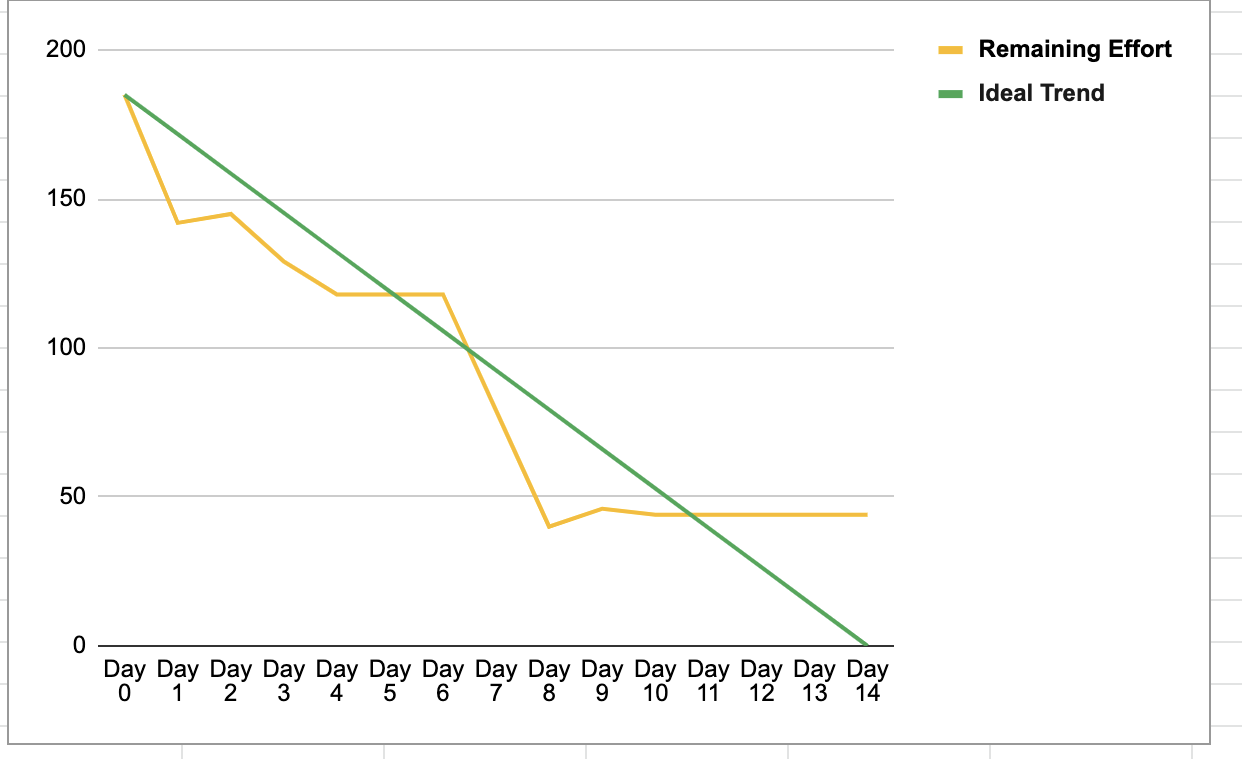
\includegraphics[scale=0.6]{pfrFigures/Sprint2.png}
    \caption{Sprint 2 Burndown chart}
    \label{fig:Burndown1}
\end{figure}

\begin{figure}[h!]
    \centering
    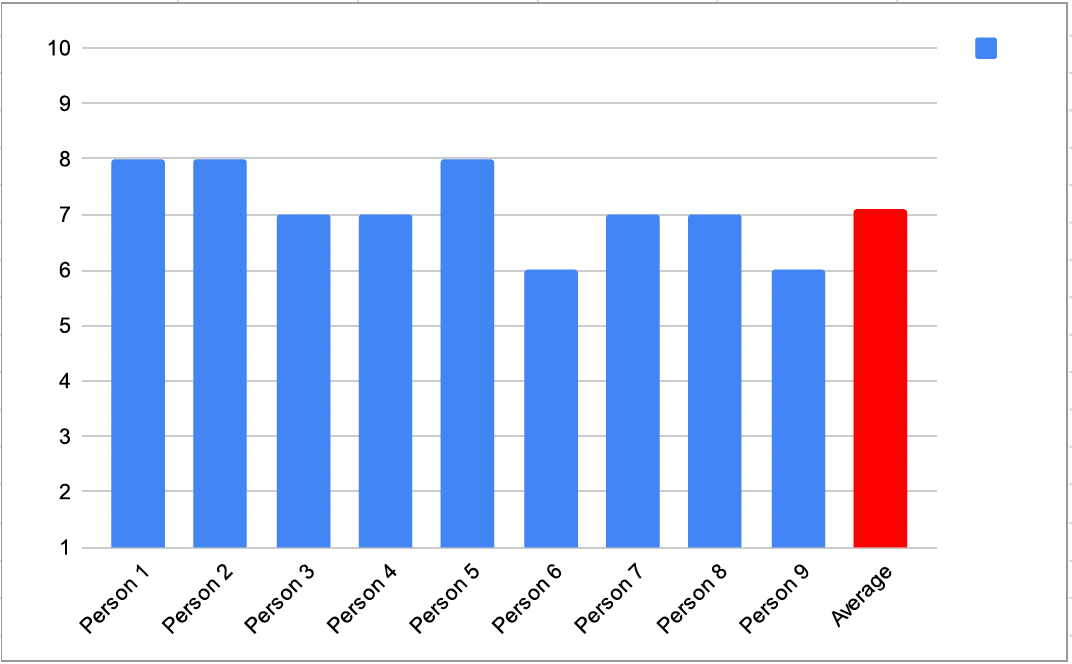
\includegraphics[scale=0.6]{pfrFigures/TeamSatisfaction2.png}
    \caption{Team satisfaction for sprint 2}
    \label{fig:Satisfaction2}
\end{figure}

\section{Phase 4} %sprint 3
\subsection{Historical overview}
We start the sprint with a sprint planning. This sprint planning is a little bit different compared to previous sprint plannings. This is because in this sprint we need to deliver a final product to the customer. Which means we now have to prioritize issues that will lead to a final product. We decided that each sub-team should meet individually and decide what type of issues they need for delivering a final product. The product owners and the scrum master then met up and labeled each issue with either "low priority", "medium priority"  or "high priority". After this the whole team met up once again. Now we needed to make sure that each functionality that back end creates, actually is implemented in front end and vice versa. All these meetings went very well and the sprint could now start. During the sprint the algorithm team raised some concerns about the algorithm. A meeting with the customer occurred. The algorithm team needed to know what the bare minimum algorithm complexity was acceptable for the customer. The meeting cleared up a lot of questions and the algorithm team could then continue to develop the algorithm. %Onsdags mötet blir vår retropsective 
During the sprint retrospective we saw that we had some problem estimating the amount of issues for this sprint. During the sprint a lot of new issues popped up as shown in Figure \ref{fig:Burndown3}. We had now also collected all the time reporting data for each sprint as shown in Figure \ref{fig:timereport} and also the data for the velocity chart as show in Figure \ref{fig:Velocity1}.From the time report we discussed that most developers felt they had a good work load and not to much or to little work to do. Some mentioned that the last sprint was a bit more hectic than the previous sprints. The scrum master also felt that he had enough work. On the o0t The overall discussion within the team was positive, we discussed how the team satisfaction improved 

%velocity chart
We can see that we now start to estimate roughly the same amount of story points. We land roughly on 200 estimated story points for a sprint. 
\subsection{Evaluation \& suggestions of improvements}
%Burndown
The reason for the new issues being added during the sprint was because of the algorithm implementation. After the meeting with the customer the teams got a better idea on what was needed for implementing the algorithm. This meant a lot of new issues appeared. Everything started when we realised that we would not be able to implement an advance algorithm in time. This meant that we needed to know what the bare minimum algorithm complexity was acceptable for the customer. This should preferably be done before the sprint, so that we could estimate those new issues in the sprint. A better planning and perhaps an earlier communications could have avoided this. At the same time we realised this at the beginning of the sprint and raised the concerns early to the customer. Unfortunately 1-2 days between each meeting makes the time go by in the sprint and before everything is resolved we are 4-5 days into the sprint. The metrics were affected negatively but in the end the algorithm got done in time and the customer was satisfied. Without the new issues this would have not been possible.

%time report
To save time for the scrum master have automatic tools for metrics. More time to help the team. Perhaps to much documentation for the project owners, would be good with a third project owner?
%velocity chart
The first sprint deviates from the  estimated story point. That is because a lot of the developers are not used to estimate and we can see that sprint 2 and sprint 3 are roughly estimated the same. This shows that the developers quickly began to learn how the estimate.

\subsubsection{The List of Forgotten Issues}

In the middle of phase 4 the product owners and scrum master found an interesting sub group of issues in the product backlog. If the issues were sorted on open issues, which were not assigned to sprint 3, the list shown in Figure \ref{fig:forgotten_issues} appeared. At first, this list appears daunting, with core functionality such as "1.2.1 Users log in using email" and "If a user is a driver, they register car brand, model, color, and licence plate".

This list of issues was shown to the team during a meeting, where it was concluded that it is a relic of multiple different things, mostly related to the ongoing attempt of using the GitLab issue tracker as an over all Scrum project management tool.

"1.2.1 Users log in using email" was an issue which was created for the PRD as this is a vital part of the product backlog. However, the login functionality was already implemented in BASE. This already closed issue was not assigned to sprint 1, nor was it closed since this would inflate the metric of the team velocity. The issue could have been revived as the transition from username -> email was implemented, but at this point, such an old issue was lost in the now much longer list of issues. The effort needed to add small issues such as this was often too great, there were a lot of steps needed for developers to properly add a new issue to the issue tracker:

\begin{itemize}
    \item Create a new issue
    \item Figure out which epic and user story the issue is associated to
    \item Give the issue an appropriate 3 number ID
    \item Add a time estimate
    \item Assign the issue a sprint, priority, and other labels
    \item Move the issue to "Doing"
    \item Do the implementation
    \item Add the time spent
    \item move the issue to "Done"
\end{itemize}

This lengthy process discouraged developers to add issues. We believe this problem would be solved by using a more advanced project management tool, which is built around the "Epics, user story, issues" structure, where adding unique identifiers and labels is not a necessity.

Big issues such as "3.1.1 Matches are made when a vehicle route is created, and it encompasses an existing passenger route" were initially in the first sprint divided into smaller issues and assigned to developers using the comment functionality. This was a way to handle the lack of a "Sub-issues" feature, but it was very bad for metrics as these sub-issues would not be recorded. Big issues like this was instead divided into smaller issues, and when they were completed the initial larger issue was forgotten. This problem would also be levitate by using an issue tracker which supports sub-issues.



\begin{figure}[]
    \centering
    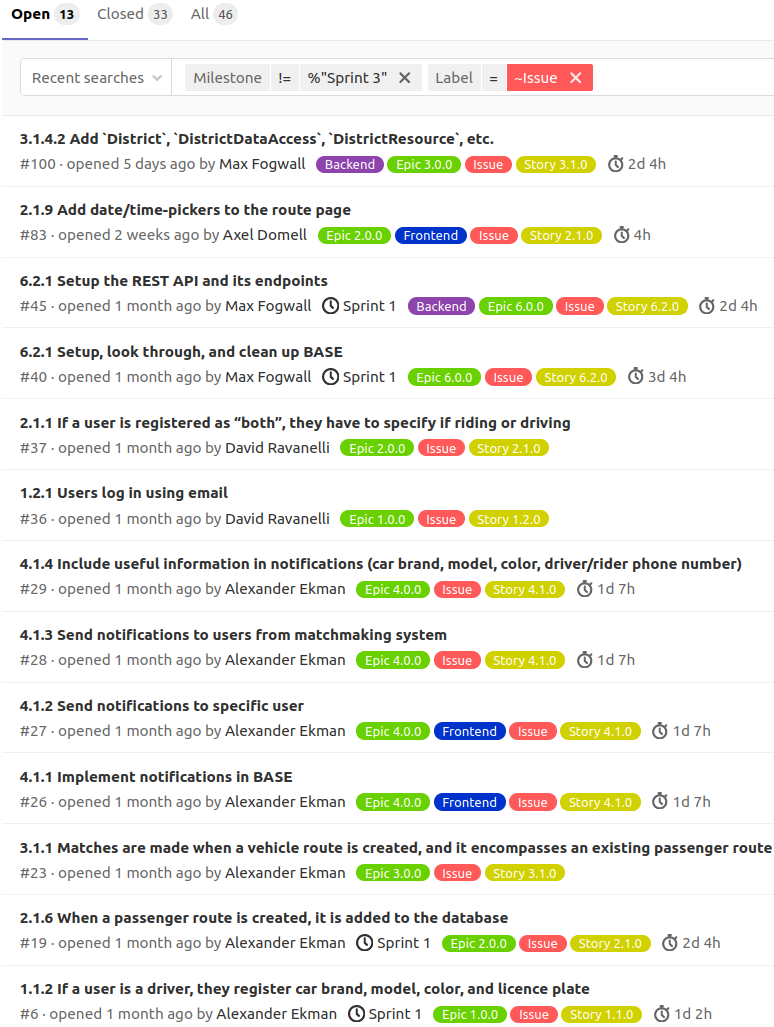
\includegraphics[scale=0.6]{pfrFigures/forgotten_issues.png}
    \caption{The list of open issues which not assigned to Sprint 3, with 1 week left of sprint 3.}
    \label{fig:forgotten_issues}
\end{figure}

\begin{figure}[]
    \centering
    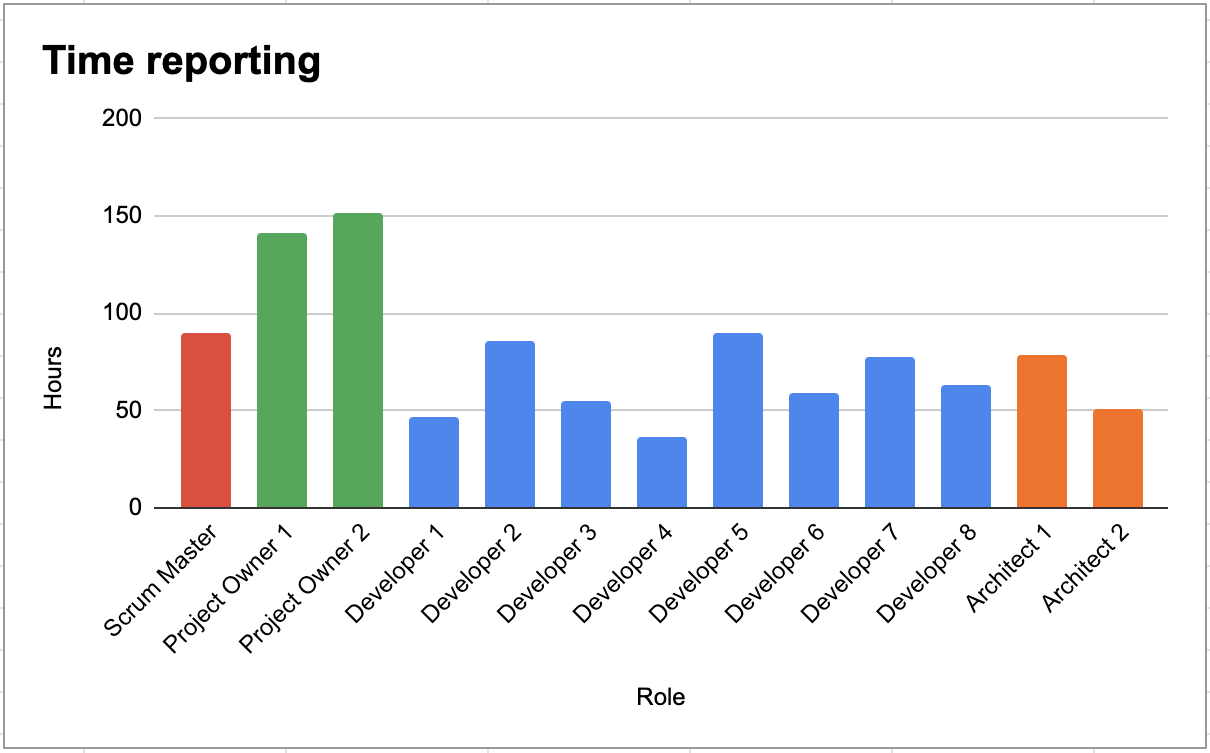
\includegraphics[scale=0.6]{pfrFigures/TimeReporting.png}
    \caption{Time spent on the three sprints combined}
    \label{fig:timereport}
\end{figure}

Instead of just dragging issues to "to-do" during sprint planning, we could assign people immediately. More product backlog grooming. Bad software.

\section{Summary and Future Outlook}

We had three main events that we had to deal with during these sprints. Firstly the underestimation of story points and amount of issues. Secondly the blocking issue and thirdly the team satisfaction. The first and second problem were dealt by tracking the metrics and then using our SDP risk analysis. The third problem was solved by using the metrics and the cooperation between the scrum master and the developers. This shows that the team followed the scrum structure and also how well the scrum method works.\newline \newline The value of the project owners was shown by the good planning and the use of their created documents, for example the risk analysis. The value of the scrum master was shown when we could track metrics and early catch when something was wrong. The metrics were then used in the sprint planning and sprint retrospective to improve the team and become better overall. The cooperation between the scrum master and the developers in scrum was also useful. This was shown when the team satisfaction problem occurred and then got resolved by the developers for sprint 3. The scrum principle of planning and then evaluating on the meetings was very useful. This was shown when the developers learned and improve their estimations after sprint 1. The developers also showed how useful they are in scrum when their good teamwork improved the metrics for each sprint.




\end{document}